\documentclass[tikz,border=8pt]{standalone}
\usetikzlibrary{arrows.meta}
\begin{document}
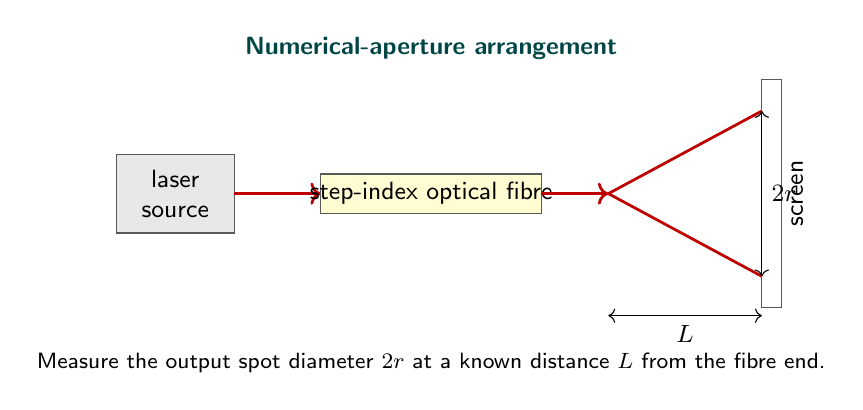
\begin{tikzpicture}[font=\sffamily\small]
\node[font=\sffamily\bfseries\small,text=teal!55!black] at (0,3.55) {Numerical-aperture arrangement};
\draw[fill=gray!18,draw=black!65] (-4,1.2) rectangle (-2.5,2.2);
\node[align=center] at (-3.25,1.7) {laser\\source};
\draw[->,red!75!black,line width=1pt] (-2.5,1.7)--(-1.4,1.7);
\draw[fill=yellow!18,draw=black!65] (-1.4,1.45) rectangle (1.4,1.95);
\node at (0,1.7) {step-index optical fibre};
\draw[->,red!75!black,line width=1pt] (1.4,1.7)--(2.25,1.7);
\draw[red!75!black,line width=1pt] (2.25,1.7)--(4.2,2.75);
\draw[red!75!black,line width=1pt] (2.25,1.7)--(4.2,.65);
\draw[fill=white,draw=black!65] (4.2,.25) rectangle (4.45,3.15);
\node[rotate=90] at (4.65,1.7) {screen};
\draw[<->] (2.25,.15)--(4.2,.15) node[midway,below] {$L$};
\draw[<->] (4.2,.65)--(4.2,2.75) node[midway,right] {$2r$};
\node[font=\sffamily\footnotesize] at (0,-.45) {Measure the output spot diameter $2r$ at a known distance $L$ from the fibre end.};
\end{tikzpicture}
\end{document}
